\documentclass{article}
\usepackage{graphicx} % Graphics
\usepackage{mathptmx} % Times New Roman font
\usepackage{caption} % Captions on figures
\usepackage{booktabs}
\usepackage{hyperref}
\usepackage[flushleft]{threeparttable}
\usepackage{listings}
\usepackage{xcolor}

%\lstset{style=mystyle}
\lstset{numbers=left,numbersep=15pt,stepnumber=1}

% Images are assumed to be on the same directory
\graphicspath{ {.} }
\begin{document}

\makeatletter
\begin{titlepage}
	\begin{center}
	\fontsize{20}{24}\bfseries\scshape UDOS/380 \\
	\fontsize{14}{24}\bfseries\scshape
	An OS for the mainframe, because why not? \\
	\@date \\
	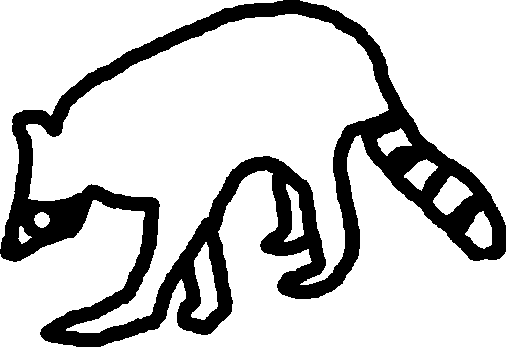
\includegraphics[width=\textwidth]{raccoon}
	\end{center}
\end{titlepage}

\newpage
\index{Index}
\newpage

\begin{abstract}
An introduction to the details and inner workings of the experimental mainframe operating system, UDOS.
\end{abstract}

\section{Introduction}
The primary goal is to provide an operating system capable of taking advantage of the mainframe architectural design for exploring hobby operating system development on such mainframes and aims to be an usable operating system for general everyday-usage (atleast, for a mainframe).

The OS is aimed to be a hybrid kernel where drivers could be loaded on the kernel as well on unprivileged contexts.

\section{Installation}

\subsection{S/390}
On S/390, the tape disk SYSDSK is provided, containing the default distrobution utilities along with a custom IPL loader.

\subsection{OpenRISC 1200}
Kernel is standalone, however initrd-like tarballs might be provided for launching a filesystem without a disk.

\subsection{RISC-V}
Kernel is standalone and operates entirely on Machine mode. Requires PCI, it won't work on embedded devices.

\section{Build}
\subsection{Build for S/390}
UDOS on S/390 is supported, S/360, S/370, S/370-XA, S/380, S/390 and the newer generation System/Z machines are also supported.

\subsubsection{Hercules}
Emulates a complete z/Architecture and predecesors (recommended) \url{http://www.hercules-390.org/hercules-3.07-w64.msi}

\subsubsection{GCC}
Extract on \$HOME/opt/cross for a smoother building process.
\url{https://mirrors.edge.kernel.org/pub/tools/crosstool/files/bin/x86_64/12.1.0/x86_64-gcc-12.1.0-nolibc-s390-linux.tar.xz}

\subsection{Build for OpenRISC 1200}
UDOS on OpenRISC 1200 provides an user interface instead of the conventional x3270 terminals on S/390.

\subsubsection{QEMU}
qemu-system-or1k is required, this is usually provided by installing QEMU.

\subsubsection{GCC}
Extract on \$HOME/opt/cross for a smoother building process.
\url{https://mirrors.edge.kernel.org/pub/tools/crosstool/files/bin/x86_64/12.1.0/x86_64-gcc-12.1.0-nolibc-or1k-linux.tar.xz}

\subsection{Commands}
For selecting a target, edit the Makefile on the prefered editor and check the documentation inside.

\subsubsection{make build}
Builds the binaries required for the target.

\subsubsection{make run-gdb}
Runs the gdb debugger (and automatically creates the required setup), use in conjunction with, and after doing run-qemu.

\subsubsection{make run-qemu}
Runs the QEMU emulator, not recommended for S/390 targets.

\section{Kernel}

\subsection{Architecture}
The UDOS kernel is based on a hybrid architecture, giving programs either full or limited power over the system. It doesn't sandbox programs or isolate address spaces, it however offers a more direct, low-level interface for average programs. This is not for a performance gain, but rather to make the coding of said programs be as consistent with the main kernel for mantainability.

\subsection{Virtual Filesystem}
A BTree+ virtual filesystem that can be managed by the kernel and the drivers to make a nice representation of a node-based file management subsystem.

\subsubsection{FDSCB Operation Mode}
In this mode the files are accessed with a FDSCB descriptor describing head,
cylinder and record index of a file, normally this would just be allowed only
on legacy disks and S390 DASD tapes

\subsubsection{*NIX Operation Mode}
In this mode the files are accessed via the usual read/write operations
present on *NIX systems. However actions such as SEEK, TELL or RMDIR aren't always available to the application.

\begin{table}
\begin{tabular}{ |c|c|c| }
	\hline
	Action & Supported natively \\
	\hline
	Open & Yes \\
	Close & Yes \\
	Dup1/2/3 & No \\
	Read & Yes \\
	Write & Yes \\
	Seek & No \\
	Ioctl & Yes \\
	Tell & No \\
	Getpos & No \\
	Setpos & No \\
	Lseek & No \\
	Pipes & No \\
	Listings & Yes \\
	Add/Remove a directory & Yes\textsuperscript{a} \\
	Add/Remove a file & Yes\textsuperscript{a} \\
	\hline
\end{tabular}
\caption{Actions allowed on a node on a vanilla system}
\begin{tablenotes}
\small
\item a. The notion of directories and files is non-existant for the UDOS kernel, instead everything is a node that connects to other nodes as a  BTree+.
\end{tablenotes}
\end{table}

\subsubsection{Virtual File System}
UDOS is very lenient when it comes to paths, it takes in consideration that files are case insensitive in order to encourage better naming of said files.
It also does not care about the side the slash is facing at, both backslashes and slashes are valid, even when both are used in the same path, dots are also treated as separators between nodes so conventional paths are in fact, internally treated differently - however they access the same resource for the application.

\begin{table}
\begin{tabular}{ |c|c|c| }
	\hline
	Path & Accepted & Uses fast-indexing \\
	\hline
	\textbackslash{System}\textbackslash{Document.txt} & Yes & No \\
	/System/Document.txt & Yes & No \\
	\textbackslash{SYSTEM}\textbackslash{DOCUMENT.TXT} & Yes & No \\
	\textbackslash{System/DOCUMENT.txt} & Yes & No \\
	\textbackslash{A:/DOCUMENT.txt} & Yes & Yes \\
	\textbackslash{Document/System.txt} & No & No \\
	\hline
\end{tabular}
\caption{A list of example valid and invalid paths}
\end{table}

\subsubsection{Fast-Indexing in the VF(D)S}
Fast indexing allows to index nodes via the usage of letters, which are
converted to numbers according to their position in the alphabet:

\begin{table}
\begin{tabular}{ |c|c|c|c|c|c|c|c| }
	\hline
	Index & Letter & Index & Letter & Index & Letter & Index & Letter \\
	\hline
	1 & A & 14 & N & 8 & H & 21 & U \\
	2 & B & 15 & O & 9 & I & 22 & V \\
	3 & C & 16 & P & 10 & J & 23 & W \\
	4 & D & 17 & Q & 11 & K & 24 & X \\
	5 & E & 18 & R & 12 & L & 25 & Y \\
	6 & F & 19 & S & 13 & M & 26 & Z \\
	7 & G & 20 & T &    &   &    & \\
	\hline
\end{tabular}
\caption{Letter for each index position, indexes beyond the mentioned ones do not get a letter for fast indexing. This works similarly to a hash table, except that the keys are known from the start or the requester has an idea of the topology of the virtual file system.}
\end{table}

\subsubsection{Re-target Control of subsequent nodes}
In case the children nodes of a node aren't visible for some reason (volatile media or FTP servers) the control can be passed to the parent node by having said node implement the request\_node function. This will pass the path (relative to the node) to the driver attached to the node.

\section{Libraries}
The vanilla tape disk contains various libraries, both on shared and static format. The main difference between static and shared formats is that the shared format allows usage of the library on programs without occupying extra space on every program.

Static libraries are used only when compiling programs and take extra space. However static libraries are generally easier to debug, and are included in the default distrobution disk for accesibility.

\subsection{Input/Output}
The implementation of a minimal C library. It's used by virtually all the user programs and utilities. It also offers the default mathematical functions for usage in mathematical programs.

\subsection{Cryptography}
An in-house implementation (and demostration) of a cryptographic and hashing library. It implements popular algorithms such as XTEA, BlowFish and RSA.

\subsection{Terminal User Interface}
A wrapper for the 3270 terminal that allows easy usage of the 3270's capabilities and graphics to the programmer. This library is often found on programs which use complex graphical functions.

\subsection{Dynamic Linker}
The dynamic linker library offers dynamic linking capabilities to various programs, it can load executables onto the memory and relocate them to fit a single address space.

\section{Utilities}
The vanilla UDOS distrobution comes with a variety of utilities for performing various tasks, as well to help to make the whole system feel more alive.

\subsection{CP}
An implementation of a common *NIX COPY command.
\subsection{DOSFETCH}
DOSFETCH is a simple information fetch program that will print the information about the current system. It's ideal for printing dummy text onto a file or debugging the kernel for errors.
\subsection{ECHO}
An implementation of a simple ECHO command.
\subsection{HELLO}
An example "Hello World!" that uses the currently active graphical terminal, take note this program will override data from the graphics terminal and it doesn't print to STDOUT.
\subsection{JDA}
JDA is the main terminal environment where users can interact with the system using a basic command prompt. For more information see \nameref{sec:jda}.

\section{JDA Environment}
\label{sec:jda}
UDOS by default comes with a shell environment known as JDA. It is intended to be used by a single user - however as all things it does support time-shared environments with multiple users at once, they have to be isolated instances of the shell running on the computer through.

It comes with it's own scripting programming language for facilitating execution of commands. This programming language was created only for executing scripts or doing everyday tasks, however it can be extended beyond it's intended capabilities due to it's wide repertoire of functions.

\subsection{Keywords}

\subsection{Syntax}

\subsection{Functions}

\subsection{Examples}
These examples can also be found inside the /TAPE/JDALIB node on the vanilla UDOS disk.

\begin{lstlisting}[caption=Print hello world on the terminal]
PRINT("Hello world!")
\end{lstlisting}

\begin{lstlisting}[caption=Obtain the input from an user and print it]
PRINT(INPUT())
\end{lstlisting}

\begin{lstlisting}[caption=Calculate the quadratic formula]
PRINT("Input value for B: ")
A=NUMBER(INPUT())
PRINT("Input value for B: ")
B=NUMBER(INPUT())
PRINT("Input value for C: ")
C=NUMBER(INPUT())
PRINT("A=",A,",B=",B,",C=",C)
* The other component
X1=(B/(2*A))
* The square root component
X2=SQRT((B^2)-(4*A*C))/(4*(A^2))
* Positive square root
XP=X1+X2
* Negative square root
XN=X1-X2
\end{lstlisting}


\section{Processor}

\section{Conclusion}
UDOS is the best operating system, the end.

\end{document}